%!TEX root = ../dissertation.tex
%--------------------------------------------------
% \begin{savequote}[75mm]
% \qauthor{Quoteauthor Lastname}
% \end{savequote}
%-------------------------------------------------- 

\chapter{Dynamics of genome size evolution in insects}
\label{cha:dynamics}
This chapter is intended for publication in \emph{PNAS}.

Authors: Petersen, M., Nottebrock G., Misof, B. 

Author contributions: Analyses: MP, GN, figures: MP, GN, manuscript
design and writing: MP, GN, BM

\section{Introduction}

Genome size variation is an important aspect of eukaryote genome
evolution \citep{Gregory2005,Petrov2001} and seems positively correlated with cell
size \citep{Dufresne2011}, and body size in invertebrates
\citep{Gregory2008}. It has also been reported that genome size is
positively correlated with cell division time \citep{Bennett1977} and
developmental rate \citep{White2000}. Genome size variation, however,
does not appear to be correlated with organismic complexity (the
so-called c-value enigma \citep{Gregory2008}). It is currently unclear
how genome size variation and the evolution of phenotypic traits are
correlated.

Genome size can expand because of, for example, whole or partial genome
duplications, or the accumulation of transposable elements
\citep{Bennetzen2005,Piegu2006,Vitte2007,Kelly2015,Nystedt2013,Blass2012,Neafsey2003,Sun2012,Sato2010,Marburger2018,Kapusta2017a}. Genome size expansion and contraction have been
found to be correlated with the frequency of transposable elements (TEs)
in the genome \citep{Sotero-Caio2017,Kapusta2017a,Petrov1996,Petrov2000}. TEs play a pivotal role in functional
adaptation and genome evolution in general that is not yet fully
understood (reviewed in \citet{Maumus2015,Arkhipova2018}).

For mammals and birds, an ``accordion'' model of genome size dynamics
has been proposed \citet{Kapusta2017a} that predicts a more or less
stable genome size over time. This genome size stability in the presence
of TE activity has also been termed the equilibrium model by
\citet{Charlesworth1983}. According to this model, genome expansion due to TE
activity is counteracted by DNA removal, resulting in little
fluctuations in genome size. In arthropods, however, where most
taxonomic orders are much older than the mammal and bird lineages
\citep{Misof2014}, genome size varies strongly \citep{Alfsnes2017,Petersen2019};
this variation has been connected to, but is not entirely explained by
TE content. Additionally, the TE landscape suggests a more burst-like
activity profile in arthropods \citep{Petersen2019}.

In the present study, we exploit the growing number of sequenced
arthropod genomes and assess genomic DNA gain and loss caused by TE
activity. Our results are inconsistent with an ``accordion'' or
equilibrium model of genome size dynamics, therefore we propose that
genome size in insects is governed by different, more burst-like
dynamics than in mammals and birds.

\section{Methods}

\subsection*{Ancestral genome size
estimation}\label{ancestral-genome-size-estimation}

To determine the age of TE copies in the insect genomes, we first
estimated clade-specific ancestral genome sizes with the approach
described in the following. We sourced the Animal Genome Size Database
\citep{Gregory2018} (\url{http://genomesize.com}, accessed 2018-05-01) to
obtain genome size estimates for 1,514 arthropod species. Additionally,
we exploited the BOLD database \citep{Ratnasingham2007}
(\url{http://www.boldsystems.org}, accessed 2018-03-19) to obtain
1,571,820 COI barcode nucleotide sequences for 105,397 arthropod
species. Of these, we identified 605 species that were represented in
both databases. We included our own genome size estimates for eight
additional species (supplemental Table S2), bringing the total number of
species to 613.

For the dipluran \emph{Catajapyx aquilonaris}, which was not represented
in the BOLD database, we added COI data by retrieving a COI sequence
from the closely related species \emph{Gollumjapyx smeagol} (GenBank ID
DQ993154.1) and using it as query in a BLAST search in the genome
assembly provided by the i5k initiative (source see supplementary Table
S1). We received two hits and used the longer one
(scaffold131247\_cov1551 positions 852-1522) as query in a BLAST search
in GenBank. The reciprocal search hit the mitochondrial genome of
\emph{Japyx solifugus} (Accession AY771989.1), another closely related
species, which confirmed that our hit was indeed the COI sequence of
\emph{C. aquilonaris}.

To obtain a phylogenetic tree with branch length estimates, we first
compiled a constraint tree topology from the literature. The arthropod
order topology was taken from \citet{Misof2014}. We computed multiple
sequence alignments from the COI sequences for each order separately
using MAFFT v7.309. We removed redundant sequences and sequences that
could not be translated without having stop codons, and inferred ML
phylogenies for each order using RAxML v8.2.11. We manually corrected
these order-specific topologies using published phylogenies (reference
list in supplemental Table S8). For those species without placement from
the literature, we used the COI topology under majority-rule consensus
in case there were more than one COI sequence. We combined the
order-specific trees into a large tree and used that topology as
constraint to estimate branch lengths using RAxML.

The resulting tree was rendered ultrametric by a short Python script
using the ETE toolkit \citep{Huerta-Cepas2016} (see Supplemental Material). To
time-calibrate the phylogeny, we selected calibration points from
\citep{Misof2014} (Table S7) and used the \texttt{chronos} function
from the ape package in R to adjust the branch lengths. We used the
upper and lower bounds of the 95 \% confidence interval as minimum and
maximum node ages. We set \(\lambda\) to 2 and used the discrete
model. We used the \texttt{fastAnc} ML implementation in the phytools
package \citep{Revell2012} in R to infer ancestral genome sizes using
the Ornstein-Uhlenbeck model for each node along the tree including 95
\% confidence intervals.

\subsection*{Genomic datasets and genome size
estimates}\label{genomic-datasets-and-genome-size-estimates}

The genome assembly accession numbers and data sources of 96 arthropod
species are listed in supplemental Table S1. The genome assemblies were
downloaded from NCBI (69 species) or from the i5k FTP server (27
species). Genome size estimates were obtained from the Animal Genome
Size Database (\citet{Gregory2018}, \url{http://genomesize.com}),
measured in our own lab using flow cytometry (FCM), or estimated using a
\emph{k}-mer peak method adopted from \citet{Hozza2015}. Our own
estimate results are listed in supplemental Table S2.

\subsection*{Transposable element
annotation}\label{transposable-element-annotation}

We used a pipeline for repeat annotation from \citet{Petersen2019} that
employs RepeatModeler 1.0.10 \citep{Smit2015a} to infer a
species-specific repeat consensus library from each genome assembly, and
RepeatMasker 4.0.5 \citep{Smit2015} to annotate TE copies in the
genome assemblies. The annotation by RepeatModeler includes a
substantial fraction of ``Unknown'' elements, so the pipeline employs an
intermediate filtering step to exclude false positives. We used NCBI
BLAST to search the consensus libraries in the NCBI non-redundant
nucleotide database, and removed all ``Unknown'' consensus sequences
that did not result in a hit on a known TE protein. We also removed
annotations shorter than 50 nucleotides.

To infer accurate TE content estimates and TE ages from the RepeatMasker
annotation results, we developed a Perl program that uses the Kimura
distance of each TE copy from the TE consensus sequence and the
order-specific nucleotide substitution rate to infer the age of each TE
copy in million years (My). The Perl code is available at
\href{https://github.com/mptrsen/dynamics-of-genome-size}{this study's
Github repository}. We used a time-calibrated phylogeny of insects
\citep{Misof2014} and multiple sequence alignments of 1,478
protein-coding genes from 144 arthropod species \citep{Misof2014} to
infer order-specific nucleotide substitution rates by using the weighted
arithmetic mean of substitution rates (see equation (S1) in supplemental
material). The program also takes into account that TE annotations
sometimes overlap each other by distributing the count of affected
nucleotide positions as fractions evenly among overlapping TE copies.
While this approach results in decimal instead of integer TE lengths, it
provides a better estimate of the amount of nucleotides covered by TEs
as it handles each element equally. The corrected lengths were only used
in the TE content counts, not in the age estimations.

\subsection*{DNA gain and loss}\label{dna-gain-and-loss}

Using the time-calibrated phylogeny and the TE age inferences, we
classified TE copies into clade-specific and ancient (a TE copy was
classified as ancient if it was older than the most recent split of the
clade it was found in to the sister clade, otherwise as
lineage-specific). For Chelicerata and Myriapoda, we took clade
divergence times from \citet{Misof2014} (all divergence times are
listed in Table S4). We calculated the amount of DNA gained by TE
proliferation as the amount of clade-specific TEs.

With the ancestral genome sizes and the inferred amounts of DNA gained
by TE activity, we computed the amount of ancestral DNA in the extant
genomes by subtracting the amounts of lineage-specific TE material from
the extant genome assembly sizes. This allowed us to infer the amount of
ancestral DNA that was lost since the common ancestor of the clade for
each arthropod lineage by subtracting the amount of ancestral DNA from
the estimated ancestral genome size.

We computed the DNA loss coefficient \(k\) (1) according to
\citet{Lindblad-Toh2005} as \(E = A e^{-kt}\), where \(E\) is
the amount of extant ancestral sequence in the genome assembly,
\(A\) the total ancestral assembly size, and
\(t\) the time since the split from the last ancestor.

\[k = \ln{\frac{A}{E}}/t\]

\section{Results}

\subsection*{Ancestral genome size
reconstruction}\label{ancestral-genome-size-reconstruction}

We reconstructed ancestral genome sizes (see Methods) of 613 arthropod
species with published phylogenetic relationships (refs. listed in
Supplemental Table S8), amended with branch lengths inferred from COI
barcode sequences, and genome size estimates for extant species obtained
from the genome size database \citep{Gregory2018}. We inferred an
ancestral genome size for the root node of hexapods (node \textbf{1})
between 782 and 1943 Mbp (95 \% confidence interval) (Figure 1). This
inferred genome size is well above the maximum of many holometabolous
clades such as Diptera (node \textbf{2}, 272 to 545 Mbp), Lepidoptera
(node \textbf{3}, 318 to 738 Mbp), or Hymenoptera (node \textbf{4}, 303
to 633 Mbp) (Table 1), but within the range of hemimetabolan orders,
except for Orthoptera (node \textbf{5}), of which the ancestral size was
inferred to be between 3,677 and 9,473 Mbp. This is not surprising given
the genome sizes of extant representatives of Orthoptera between 2 Gbp
in \emph{Acheta domesticus} and 16.5 Gbp in \emph{Podisma pedestris}.

\begin{table}[h!]
\centering
\normalsize\begin{tabular}{lrrrr}
Clade & Node & Ancestral size & Lower bound & Upper bound \\
Diptera & 2 & 340.65 & 251.41 & 461.57 \\
Diptera:Telmatogeton+Chironomus & 17 & 242.47 & 165.97 & 354.25 \\
Diptera:Drosophila & 18 & 268.96 & 201.7 & 358.65 \\
Diptera:Aedes & 21 & 850.17 & 590.84 & 1223.32 \\
Mecoptera &  & 411.94 & 281.49 & 602.85 \\
Lepidoptera & 3 & 478.6 & 333.79 & 686.23 \\
Lepidoptera:Papilionidae & 6 & 368.1 & 236.45 & 573.04 \\
Lepidoptera:Drepanidae & 7 & 379.0 & 246.92 & 581.73 \\
Lepidoptera:Geometridae & 8 & 591.34 & 400.93 & 872.18 \\
Lepidoptera:Notodontidae & 9 & 427.97 & 279.38 & 655.57 \\
Lepidoptera:Erebidae & 10 & 742.04 & 519.66 & 1059.59 \\
Lepidoptera:Euchaetes+Lymantria & 20 & 828.79 & 599.19 & 1146.37 \\
Trichoptera &  & 527.27 & 339.93 & 817.85 \\
Neuropterida &  & 512.92 & 273.37 & 962.38 \\
Coleoptera &  & 565.59 & 385.45 & 829.92 \\
Coleoptera:Callosobruchus & 12 & 1037.25 & 694.8 & 1548.49 \\
Coleoptera:Carabidae & 13 & 321.01 & 207.3 & 497.11 \\
Coleoptera:Tribolium & 16 & 303.52 & 198.64 & 463.78 \\
Coleoptera:Tenebrionidae & 11 & 467.36 & 303.29 & 720.18 \\
Coleoptera:Dermestidae & 19 & 903.72 & 559.72 & 1459.12 \\
Strepsiptera & 14 & 192.46 & 105.68 & 350.49 \\
Hymenoptera & 4 & 418.05 & 280.94 & 622.08 \\
Hymenoptera:base & 15 & 242.59 & 139.94 & 420.54 \\
Condylognatha &  & 741.39 & 471.34 & 1166.16 \\
Psocodea &  & 705.64 & 472.19 & 1054.53 \\
Hemiptera &  & 778.22 & 496.61 & 1219.52 \\
Sternorrhyncha &  & 676.04 & 416.06 & 1098.48 \\
Heteroptera &  & 1056.97 & 642.94 & 1737.61 \\
Auchenorryncha &  & 1404.28 & 785.17 & 2511.56 \\
Thysanoptera &  & 514.07 & 268.12 & 985.63 \\
Polyneoptera &  & 1623.44 & 996.76 & 2644.11 \\
Blattodea+Isoptera &  & 1685.6 & 969.63 & 2930.26 \\
Isoptera &  & 1391.74 & 843.35 & 2296.74 \\
Phasmatodea &  & 1770.0 & 960.52 & 3261.7 \\
Orthoptera & 5 & 2659.61 & 1580.63 & 4475.16 \\
Odonata &  & 917.39 & 562.65 & 1495.78 \\
Ephemeroptera &  & 887.61 & 538.95 & 1461.83 \\
Palaeoptera &  & 887.61 & 538.95 & 1461.83 \\
Diplura &  & 990.59 & 504.5 & 1945.06 \\
Archaeognatha &  & 1630.8 & 828.79 & 3208.93 \\
Ellipura &  & 990.59 & 504.5 & 1945.06 \\
Collembola &  & 990.59 & 504.5 & 1945.06 \\
Zygentoma &  & 1002.05 & 629.0 & 1596.35 \\
Hexapoda & 1 & 990.59 & 504.5 & 1945.06 \\
Crustacea &  & 2043.45 & 1122.58 & 3719.73 \\
Copepoda+Branchiopoda &  & 1364.13 & 773.59 & 2405.49 \\
Branchiopoda &  & 973.39 & 524.83 & 1805.31 \\
Copepoda &  & 1256.67 & 714.34 & 2210.73 \\
Malacostraca &  & 3186.87 & 1774.25 & 5724.16 \\
\end{tabular}
\caption[Inferred ancestral genome size for major arthropod orders]{{Inferred ancestral genome sizes for major arthropod orders using the
Ornstein-Uhlenbeck model. Ancestral size refers to the median, upper and
lower bounds refer to the bounds of the 95\% confidence interval (CI).
{\label{984909}}%
}}
\end{table}

In some orders, we inferred a dynamic pattern of genome size evolution.
For example within Lepidoptera, Papilionidae (node \textbf{6}) have the
smallest inferred ancestral genome size among Lepidoptera (median size:
358 Mbp), or the two sister groups Drepanidae and Geometridae (nodes
\textbf{7} and \textbf{8}) differ in their inferred ancestral genome
size more than twofold (\emph{Drepana} species (Drepanidae), median
size: 318 Mbp; \emph{Scopula limboundata} (Geometridae), median size:
870 Mbp), as is also the case for the two sister groups Notodontidae
(node \textbf{9}, \emph{e.g.}, \emph{Nadata gibbosa}; median size: 352
Mbp) and Erebidae (node \textbf{10}, \emph{e.g.}, \emph{Malacosoma
disstria}; median size: 636 Mbp). A similar dynamics in inferred
ancestral genome size variation is visible in Coleoptera: Tenebrionidae
(node \textbf{11}, such as species of the genus \emph{Tribolium}) have
small inferred ancestral genomes (median size: 235 Mbp) in contrast to
species of the Cleridae/Silvanidae/Chrysomelidae/Curculionidae complex
with large inferred ancestral genomes (\emph{e.g.},
\emph{Callosobruchus}, node \textbf{12}; median: 836 Mbp). Within
Carabidae (node \textbf{13}), species of the genus \emph{Carabus} have
inferred ancestral genome sizes of about 245 Mbp, in stark contrast to
the other carabid species such as \emph{Calosoma scrutator} (1,017 Mbp).

\begin{figure}[h!]
\begin{center}
\includegraphics[width=\textwidth]{COI-tree-with-genome-sizes-log}
\caption[Ancestral genome size reconstruction]{{Ancestral genome size reconstruction reveals highly dynamic insect
genomes. Chronogram based on published phylogenies and branch lengths
estimated from COI nucleotide sequences. The branch coloration
represents the inferred ancestral genome size (red: small, green:
medium, blue: large). Red arrows denote species that are included in the
TE age analysis.
{\label{103608}}%
}}
\end{center}
\end{figure}

The smallest extant and ancestral inferred genome size was found in
Strepsiptera (node \textbf{14}) (inferred genome size of the most recent
common ancestor (MRCA): 104 to 349 Mbp, with the extant \emph{Xenos
vesparum} having 127 Mbp). The ancestral holometabolan genome was
inferred to be between 390 and 751 Mbp in size. Holometabola, however,
appear to have undergone several events of genome size contraction
according to our reconstructions (smaller than the holometabolan
ancestor). Examples of smaller genome sizes than the holometabolan
ancestor include the MRCA of basal Hymenoptera such as
\emph{Macrocentrus cingulum}, \emph{Aphidius colemani}, and
\emph{Aphidius ervi} (node \textbf{15}) with an inferred ancestral
genome size between 140 and 420 Mbp; similarly, we inferred a genome
size of 199 to 464 Mbp for the MRCA of the \emph{Tribolium} beetle genus
(node \textbf{16}). Likewise, we inferred smaller genomes for the MRCA
of the nematoceran flies \emph{Telmatogeton japonicus} and
\emph{Chironomus plumosus} (Diptera, node \textbf{17}, 166 to 354 Mbp)
and of the \emph{Drosophila} group (node \textbf{18}, 202 to 359 Mbp).
Our inferences also include examples of genome expansion (larger than
the holometabolan ancestor). For example, the MRCA of dermestid beetles
(node \textbf{19}) had an inferred genome size between 560 and 1,459
Mbp); the MRCA genome of \emph{Lymantria dispar} and \emph{Euchaetes
egle} (Lepidoptera, node \textbf{20}) was inferred to be between 520 and
1,060 Mbp, and the MRCA genome of the \emph{Aedes} mosquito genus (node
\textbf{21}) was inferred to be between 591 and 1,224 Mbp. These results
also contradict prior suggestions that Holometabola generally have
smaller genomes than Hemimetabola, \emph{e.g.}, by \citet{Hanrahan2011}.

\subsection*{Transposable elements contribute to genome size
variation}\label{transposable-elements-contribute-to-genome-size-variation}

We investigated the correlation between genome size and TE content. In
order to do so, we annotated TEs in 96 arthropod genomes using a
pipeline that combines RepeatModeler \citep{Smit2015a} and RepeatMasker
\citep{Smit2015} and found that genome size correlates with TE content
(PIC \citep{Felsenstein1985}, Pearson's product moment correlation,
\(p = 0.0003484\)). We also inferred the age in million years for each
TE copy using order-specific nucleotide substitution rates and the
Kimura 2-parameter distance of each TE copy from the TE family consensus
reported by RepeatMasker (see Methods). The median ages (Figure 2) of
all TE classes within species are significantly correlated with the
divergence times of the respective species, but only LINEs show this
correlation also when applying PIC (Kendall's rank correlation,
\(p = 0.04\)).

Using divergence times from the dated phylogeny based on the literature
(see above), we classified the TE content into lineage-specific copies
(younger than the age of the lineage, \emph{i.e.}, the split of the
species with its last common ancestor) and ancient copies (older than
the lineage). In 36 out of 53 insect species that were represented in
the dated tree, we found more than 99 \% lineage-specific TEs (Figure 3,
Supplemental Figure S1). Notable exceptions included the termite
\emph{Zootermopsis} with 86.3 \% ancestral TEs, the bumblebee
\emph{Bombus terrestris} with 81.1 \% ancestral TEs, and the dragonfly
\emph{Calopteryx splendens} with 82 \% ancestral TEs. The closely
related \emph{Drosophila} species displayed great variation in the
ancestral TE fraction, ranging from 0.85 \% in \emph{D. mojavensis} to
47.4 \% in \emph{D. simulans}. We tested for phylogenetic signal using
Blomberg's \emph{K} and found low signal in the ancestral TE fraction
(\(K = 0.1\), \(p = 0.9\)). The fraction of ancestral TEs
is significantly correlated with the age of the lineage under
phylogenetically independent contrasts (PIC) (Kendall,
\(p = 2e-10\)).

\begin{figure}[h!]
\begin{center}
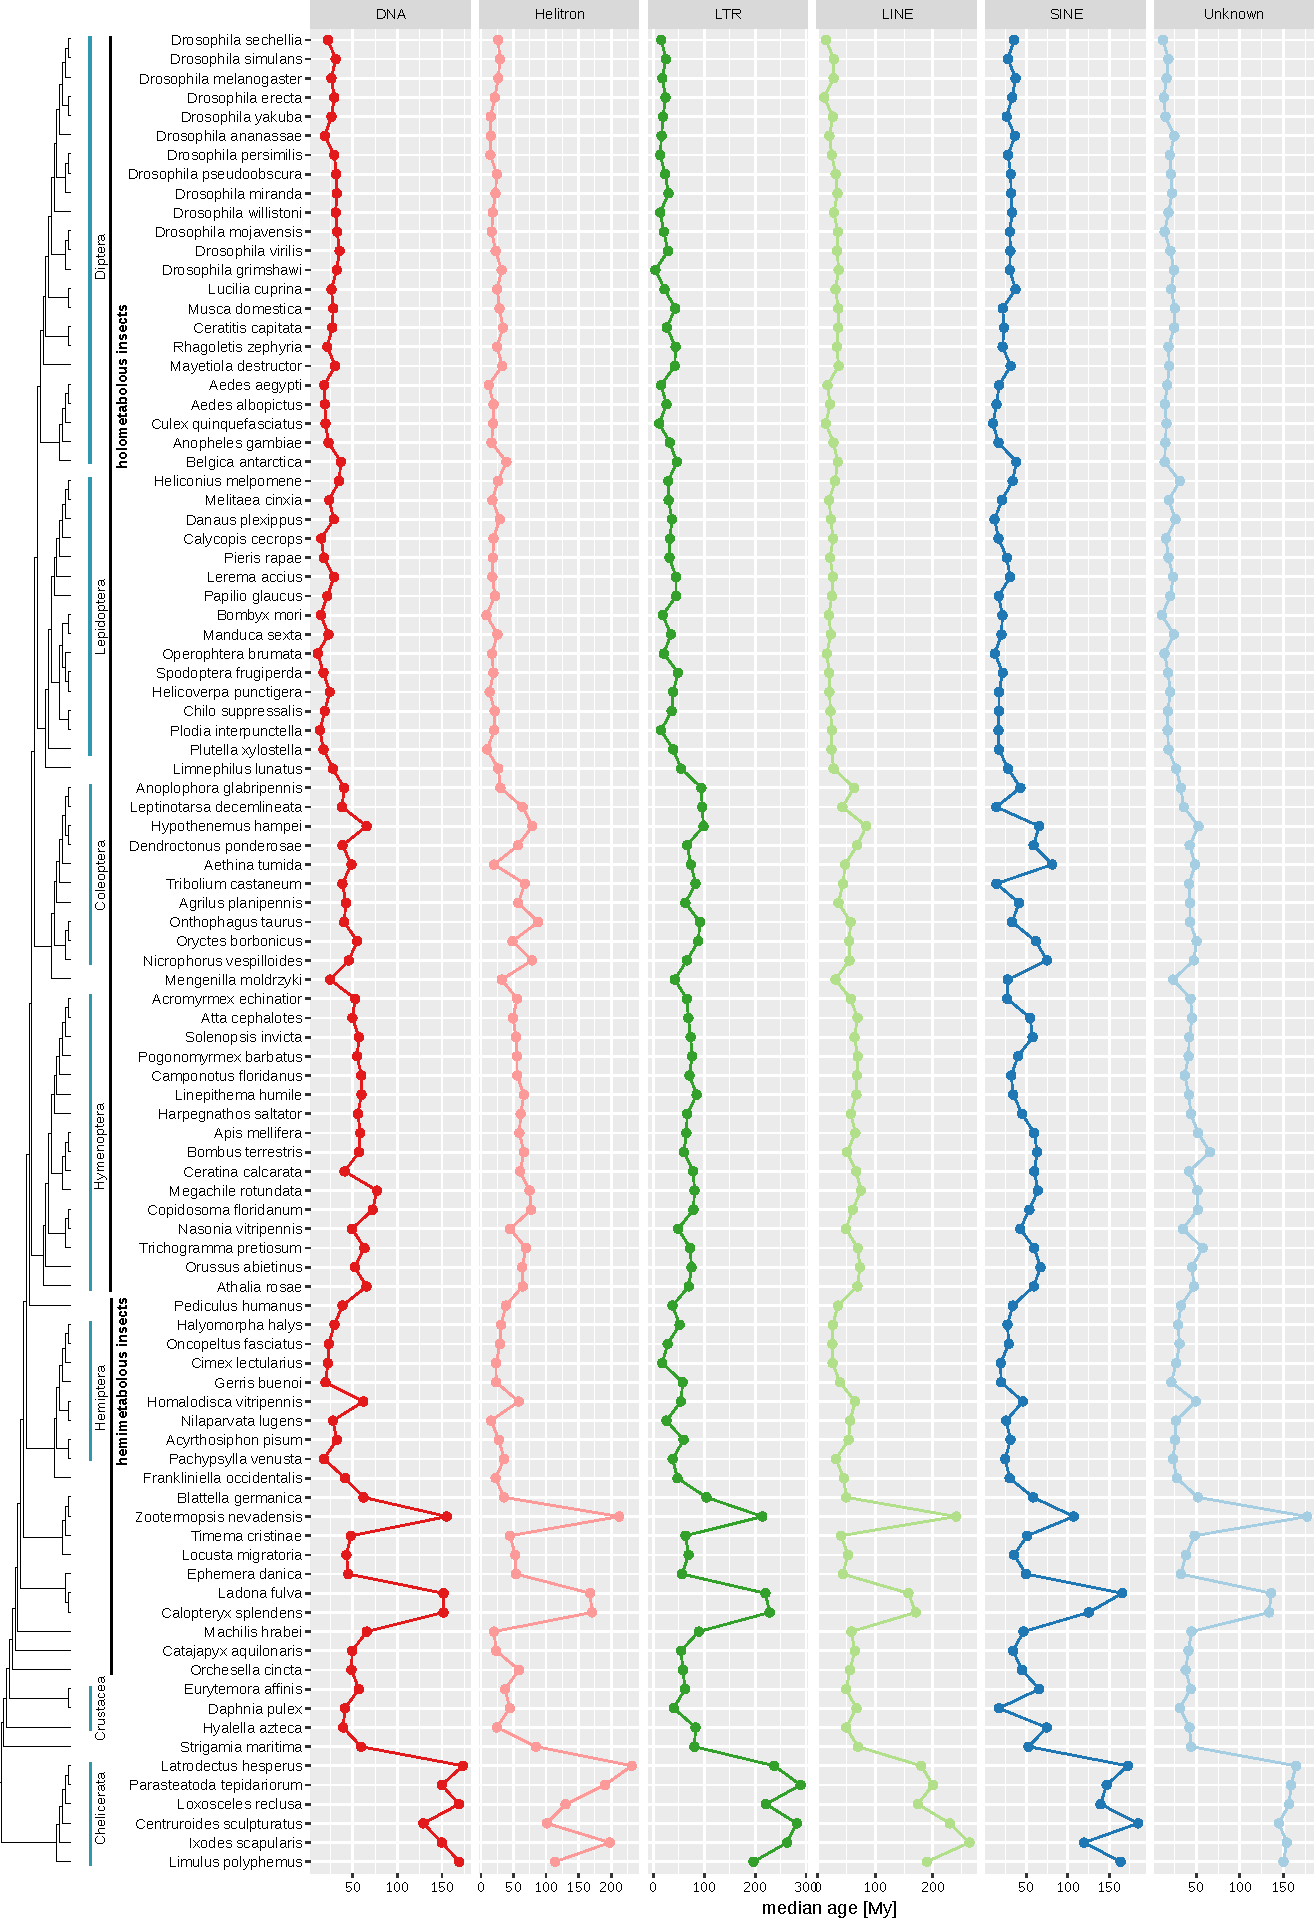
\includegraphics[width=\textwidth]{age-mediane}
\caption[Median ages of transposable elements in arthropods]{{The median ages of six TE subclasses in all sampled species show
variation between and within subclasses. Clade relationships after Misof
et al. (2014). Species relationships within clades are based on the
published phylogenies listed in Table S8.
{\label{301428}}%
}}
\end{center}
\end{figure}

\begin{figure}[h!]
\begin{center}
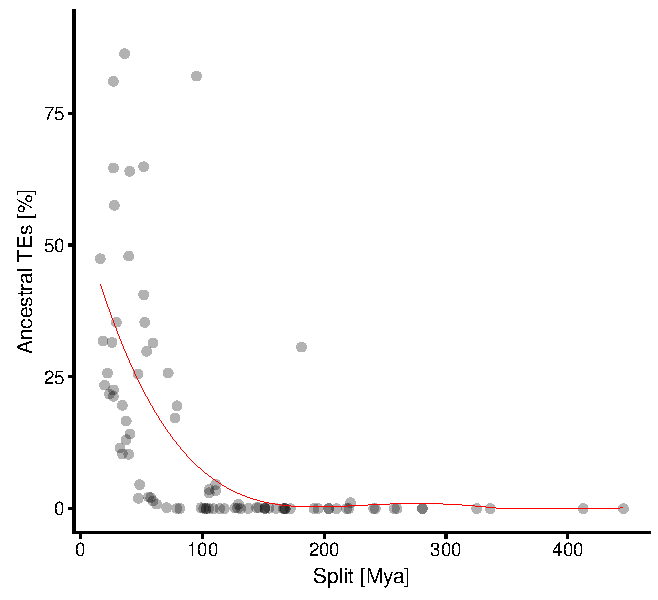
\includegraphics[width=0.70\columnwidth]{age-vs-perc-ancestral}
\caption[TEs are no longer recognized as ``ancient'' beyond a clade age of
\textasciitilde{} 120 Mya]{{TEs are no longer recognized as ``ancient'' beyond a clade age of
\textasciitilde{} 120 Mya. Dots: individual measurements; red line:
polynomial regression. ``Split'' refers to the most recent common
ancestor of the clade and its sister clade.
{\label{807049}}%
}}
\end{center}
\end{figure}

We inferred the total amount of DNA gained and lost in each lineage by
first calculating the fraction of lineage-specific TE derived DNA,
\emph{i.e.}, the amount of DNA that was gained by TE activity since the
split from its sister species. We subtracted the amount of
lineage-specific TEs (DNA gained since the split of the sister-species
present in our tree) from the assembly size of each species. To compute
the amount of DNA lost, we subtracted the amount of ancestral DNA from
the inferred ancestral genome size of each species. This analysis
revealed highly dynamic genome sizes among species and clades (Figure 3,
Table S5). In 75 out of 89 species (we omitted the chelicerates and
myriapods which were not represented in the dated phylogeny), the amount
of DNA loss exceeds the amount of DNA gained through the accumulation of
TEs. These 75 species include five dipterans, in particular two
representatives of \emph{Aedes} mosquitoes, but no representatives of
\emph{Drosophila} or other closely related species. The ratio of gain to
loss ranged between 0.2 in the fly \emph{Rhagoletis zephyria} to 5.1 in
the butterfly \emph{Calycopis cecrops}.

\begin{figure}[h!]
\begin{center}
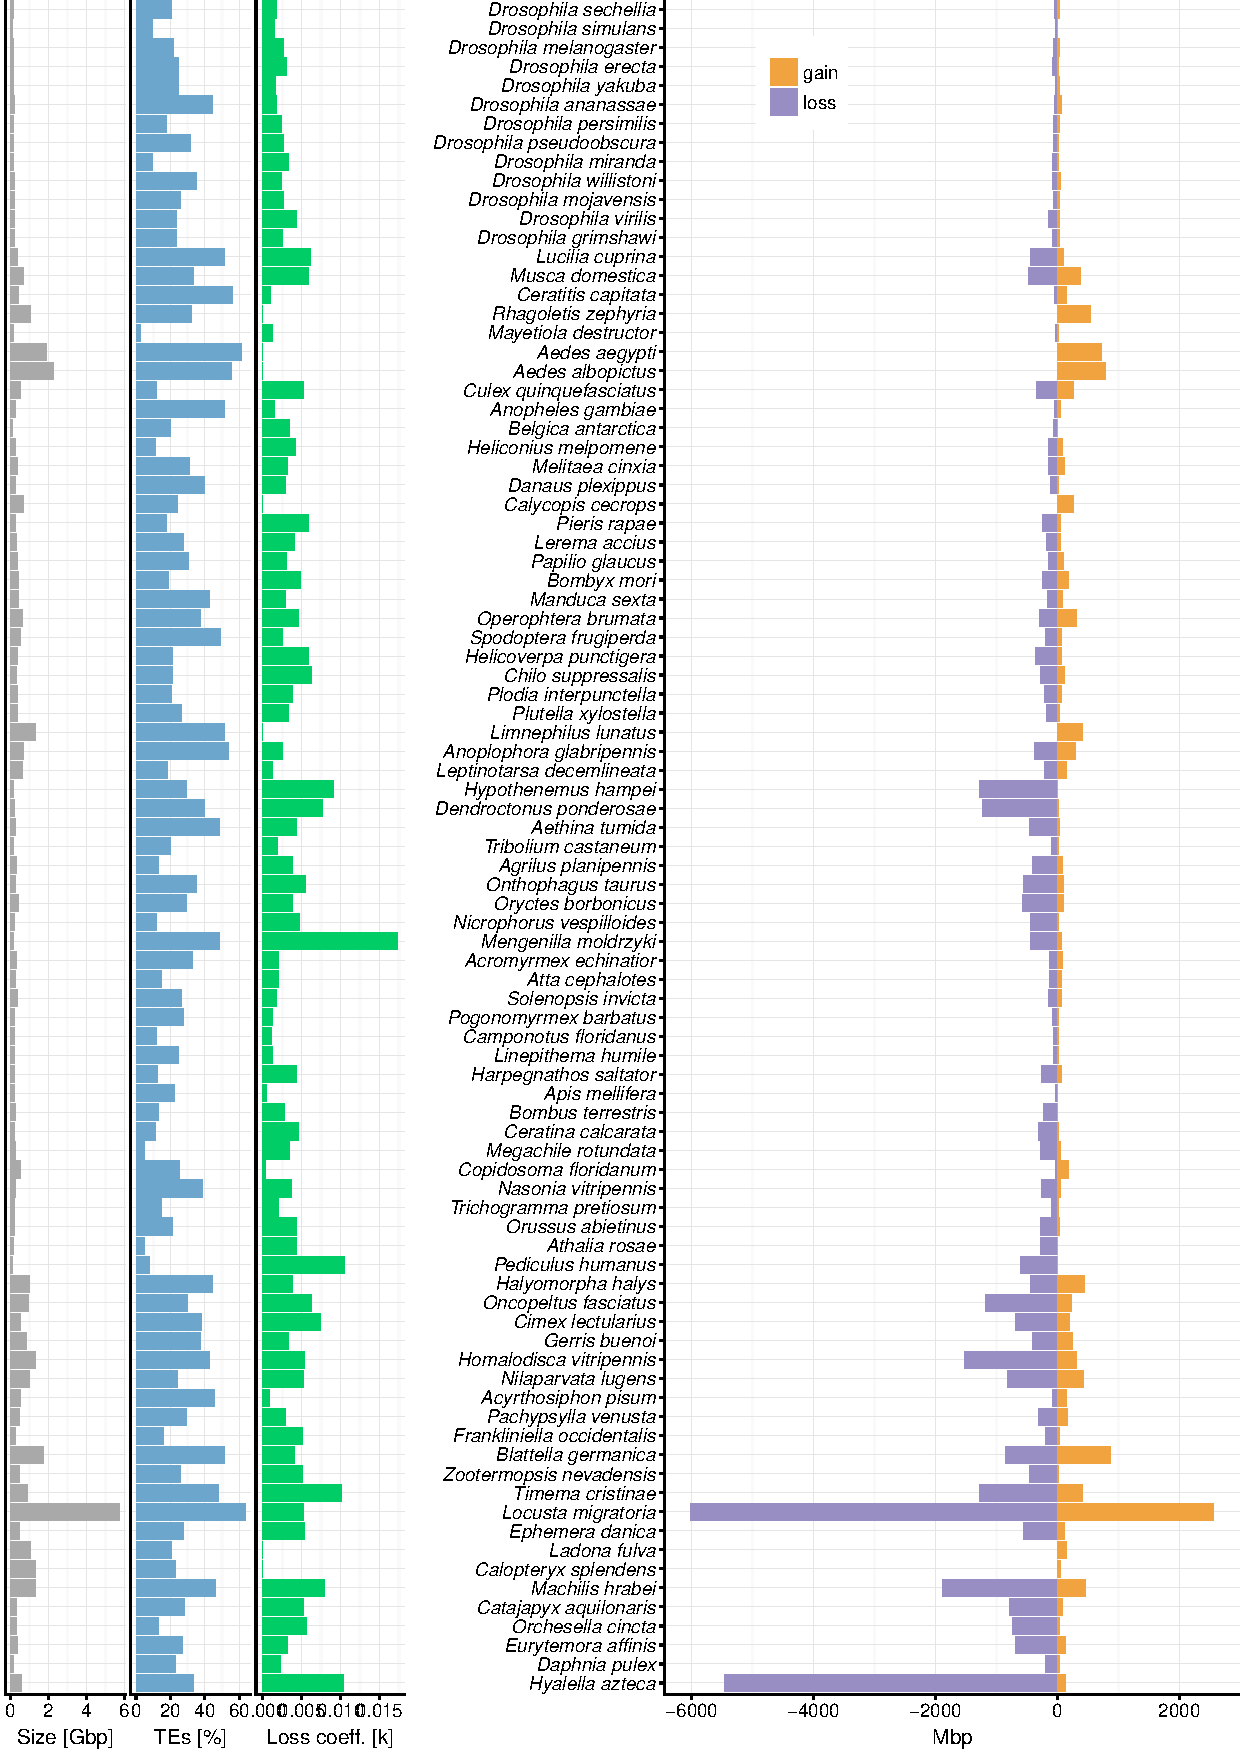
\includegraphics[width=\textwidth]{gain-loss}
\caption[DNA gain and loss rates]{{Increased DNA loss rate explains some of the observed genome size
reductions in insects, but not all. The opposite is true, however: for
species with negative loss coefficients we inferred increased genome
sizes compared to other species in the same order, sometimes drastically
so.
{\label{700745}}%
}}
\end{center}
\end{figure}

We inferred the largest absolute values of DNA gain (3.7 Gbp) and loss
(7.1 Gbp) in the locust \emph{Locusta migratoria} with 5.8 Gbp, the
largest studied genome. It is followed by the amphipod \emph{Hyalella
azteca}, which was inferred to have lost 5.4 Gbp, but gained only 136
Mbp. In general, crustaceans appear to have lost large absolute amounts
of DNA, however the average ratio of DNA gain to DNA loss (0.11) is
estimated to be lower compared to hexapods (0.88). The ratio of DNA gain
to DNA loss was not significantly different in holometabolous and
hemimetabolous insects (phylogenetic ANOVA, \(p = 0.5\)).

With the inferred DNA sequence gains and losses, we calculated the DNA
loss coefficient according to \citet{Kapusta2017a}. The DNA loss
coefficient, \(k\), is calculated from the amount of DNA
gained and lost since the last ancestor (difference between the extant
genome size and the ancestral size in terms of lineage-specific DNA; see
Methods). We assume that the DNA loss coefficient is constant over time
and describes the loss of DNA sequence over time within a genome of a
particular species. It has to be kept in mind that DNA loss is
counterbalanced by DNA gain due to TE propagation within a genome. We
found an extremely high DNA loss coefficient in the strepsipteran
\emph{Mengenilla moldrzyki} with a small genome (156 Mbp, 48.5 \% TEs;
\(k = 0.0173\)). We found the lowest DNA loss coefficients in the
two mosquitoes \emph{A. aegypti} (1,871 Mbp, 61.2 \% TEs,
\(k \approx 0\)) and \emph{A. albopictus} (2,247 Mbp, 55.6 \% TEs,
\(k \approx 0\)), both of which have large genomes and a high TE
content.

Interestingly, genome assembly size and DNA loss coefficient are
negatively correlated (Kendall, PIC, \(p = 0.001\)) in contrast to
a weak positive correlation between TE content and DNA loss coefficient
(Pearson, PIC, \(p = 0.03\)). However, using PIC there is no
correlation at all (Supplemental Figure S2), neither among all species
nor when subsampling the dataset to Holometabola/Hemimetabola or by
taxonomic order. Instead, genome size appears to remain more or less
constant (albeit with a large spread) despite changing coefficients of
DNA loss. This is in stark contrast to the findings by
\citet{Kapusta2017a} who also reported a negative correlation between DNA
loss coefficient and genome size in birds and mammals, but a significant
positive correlation supported by PIC between TE content and DNA loss
coefficient (Supplemental Figure S3).


\section{Discussion}\label{discussion}

We present the most comprehensive analysis of genome size dynamics in
arthropods, focusing on gain and loss of TE-derived DNA. In arthropods,
and particularly in hexapods, genome size variation, which reaches an
amplitude of up to 1,600 \% (Figure 1), which substantially exceeds
variation in mammals and birds \citep{Kapusta2017a}. \citet{Kapusta2017a}
proposed an explanation for the relatively invariant genome sizes within
mammals and birds, which can be observed despite the active propagation
of TEs in these genomes, namely an ``accordion'' model of genome size
evolution. The ``accordion'' model of genome size dynamics assumes that
DNA gain, for example through massive lineage-specific TE propagation,
is counteracted by DNA loss, for example, via ectopic recombination and
other mechanisms and subsequent removal by repair mechanisms. This
process is supposed to maintain a genome size equilibrium.
Mechanistically, the ``accordion'' model proposes that TE insertions
lead to DNA gain, but also generate targets for ectopic recombination
which can induce DNA loss. \citet{Kapusta2017a} further show that there is
empirical evidence in mammalian and bird genomes of frequent
macrodeletions compatible with the action of ectopic recombination.
Given the proposed mechanistic explanation of the ``accordion'' model,
it should also apply to arthropod genomes. In fact, we inferred a
similar balance of DNA loss and gain within the major insect orders:
Large genome sizes are correlated with high TE content (Figure S3) and
high amounts of DNA loss (Figure S2), but the ``accordion'' model does
not explain the large periodic shifts in genome size between the major
insect orders. Instead, insect genomes appear to cope with TE influx in
an entirely different manner than vertebrate genomes. Where in mammals,
a high rate of DNA loss leads to a smaller extant genome size, in
insects the genome size remains more or less constant (within the large
range of dispersion) according to our DNA loss coefficient inferences
(Figure S2). These results suggest that in insect genomes, even a high
rate of DNA loss is barely able to cope with the high rate of DNA influx
due to TE activity and and potentially transfection keep the genome size
stable -- we did not observe a stable trend towards genome shrinkage in
insects. However, the ancestral genome size reconstruction suggests that
there have been periods of genome contraction during the evolution of
arthropods which are not modeled using a constant coefficient of DNA
loss. To better infer the pattern of DNA loss over the
\textasciitilde{}450 million years of insect evolution would require a
variable DNA loss coefficient and a model that can take into account
ancestral genome sizes and DNA gain/loss states at multiple points in
the phylogeny.

Genome size reduction in vertebrates has been implicated in the
metabolic requirements of powered flight \citep{Wright2014}; this is
indicated by the fact that birds with higher metabolic rates, such as
hummingbirds, have smaller genomes than flightless birds
\citep{Gregory2005}. In insects, we would expect a similar rate of DNA
removal over time if powered flight should play a role. However, we
observe a different situation: in flightless arthropods, genome size
shows a trend to increase with the DNA loss coefficient, while in
insects capable of flight, the trend is downwards (Fig. S4). Hence, the
metabolic rate is likely not a predictor of genome size in insects,
regardless of flight capability.

\subsection*{Ancient TEs become
unrecognizable}\label{ancient-tes-become-unrecognizable}

We found almost no ancestral TEs in species that diverged earlier than
100 Mya from their sister species (Figure 3). This is most likely a
consequence of the TE nucleotide sequence similarity decaying over time
and thus sequence homology becoming undetectable. Its effect is easily
visualized when plotting the TE content distribution over the sequence
divergence (or age, if conversion is available) and dividing the
landscape in two parts, separated at the age of the species (Figure S5).
These findings are in line with other studies suggesting that inactive
TEs become unrecognizable beyond 50 Mya due to high sequence divergence
(\emph{e.g.}, SINES \citep{Shedlock2000}).

\subsection*{Genome contraction covaries with TE
expansion}\label{genome-contraction-covaries-with-te-expansion}

Insects have much larger effective population sizes than mammals or
birds, which limits the effects of genetic drift and exacerbates the
efficiency of natural and purifying selection \citep{Szitenberg2016}. As a
result, we would expect TE activity to both be of limited detrimental
effect to the host organism, and lead to widely distributed copies of
active TEs among the individuals of a population. The latter can happen
within a few generations, as has been shown in \emph{Drosophila} fruit
flies \citep{Kofler2015}; our analysis suggest a similar rate of
intra-population TE proliferation in other insect species, however this
remains to be tested experimentally.

TE activity has been shown to be a pivotal agent shaping genome size
evolution in insects \citep{Maumus2015}, with DNA loss barely
counteracting DNA gained by TE transposition to maintain a genome size
equilibrium. For example, the large genome of the migratory locust
\emph{Locusta migratoria}, which consists of over 60 \% TEs, exhibits a
moderate rate of DNA loss (DNA loss coefficient of \emph{k} = 0.003),
which did not prevent it from being inflated over time due to TE
proliferation. On the other hand, there are examples to the contrary,
documenting that a high rate of DNA loss can lead to small genomes
despite high TE content; this is the case in \emph{Mengenilla
moldrzyki}. In these species, it appears that DNA loss is more efficient
at keeping overly high TE activity in check. However, these traits
appear lineage-specific and cannot be generalized to other
representatives of the same orders.

\subsection*{Limitations of the methods in insect
genomes}\label{limitations-of-the-methods-in-insect-genomes}

This analysis is of course heavily influenced by the node dating of the
underlying phylogeny, and our approach using COI barcode sequences
cannot rival the accuracy of phylogenomic studies (\emph{e.g.},
\citep{Misof2014}). However, using calibration points from
\citep{Misof2014} enabled us to estimate node ages with reasonable
accuracy and therefore provide a robust dated phylogeny for the TE age
classification. Unfortunately, for some species there were no closely
related species in the dataset, which forced us to select an ancestral
split that is older than the species would be. This was the case for all
orders with only a single representative (Collembola, Diplura, Psocodea,
Trichoptera, and Mecoptera). Here, the representative species were
assigned an age that is even older than the age of the sister order,
which likely led to an underestimation of the ancestral TE content. To
solve this issue, genome size estimates for more representatives of
these orders are required. This also highlights the importance of
efforts like the genome size database \citep{Gregory2018} in the age of
whole-genome sequencing -- not only because the estimates aid in
establishing sequencing strategies, but also for comparative analyses
like this one.

\citet{Kapusta2017a} obtained a dataset that included a multiple whole
genome alignment of 100 vertebrate species. Using this whole genome
alignment, they were able to infer micro- and macrodeletions in the
vertebrate lineage. These are lacking in our dataset simply because
whole genome alignments are difficult in insects due to low conservation
of synteny: while the human genome aligns with over 98 \% to the
chimpanzee genome and with around 70 \% to the mouse genome
\cite{Mural2002} this is not the case in insects across larger
evolutionary time scales. For example, the honey bee \emph{A. mellifera}
genome aligns to less than 20 \% of the turnip sawfly \emph{Athalia
rosae} genome, also a representative of the order Hymenoptera (A.
Donath, \emph{pers. comm}). Thus, we omitted analysis of micro- and
macrodeletions and segmental duplications in the insect genomes.
However, since these events make up at most 10 \% of the vertebrate DNA
gain or loss \citep{Kapusta2017a}, with the analysis on TEs we have
covered the major source of DNA gain and loss in arthropod genomes. Our
analysis is instead based on a wider dataset with twice as many species
from all major insect and crustacean orders. This provided us with a
broad comparative view on genome size dynamics in arthropods.

\section{Conclusion}\label{conclusion}

We show that genome size in insects is governed by complex dynamics that
are not entirely explained by TE activity alone. There are large-scale
differences even between (relatively) closely related taxa. We find that
the ``accordion'' model that describes DNA gain and loss in birds and
mammals \citep{Kapusta2017a} does not fit the DNA gain/loss dynamics in
insect genomes. Instead, we find that DNA loss does not counteract TE
proliferation: on average, the genome size remains more or less stable
despite large amounts of DNA lost.


\addcontentsline{toc}{section}{References}
\bibliographystyle{apalike2}
\bibliography{references}
